\documentclass{standalone}
\usepackage{tikz}
\usepackage{ctex,siunitx}
\setCJKmainfont{Noto Serif CJK SC}
\usepackage{tkz-euclide}
\usepackage{amsmath}
\usetikzlibrary{patterns, calc,3d}
\usetikzlibrary {decorations.pathmorphing,decorations.pathreplacing,decorations.shapes}
\begin{document}
\small
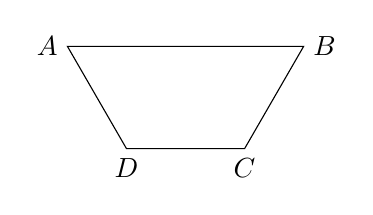
\begin{tikzpicture}[>=latex,scale=1.0]
  \draw(-0.75,0)node[below]{$D$}--(0.75,0)node[below]{$C$}--++(60:1.5)node[right]{$B$}--++(-3,0)node[left]{$A$}--cycle;
\end{tikzpicture}
\end{document}